\documentclass[11pt]{article}
\usepackage[utf8]{inputenc}\usepackage[T1]{fontenc}
\usepackage{amsmath,amssymb,amsthm}\usepackage[margin=1in]{geometry}
\usepackage{graphicx}\usepackage{booktabs}\usepackage{multirow}
\usepackage[hidelinks]{hyperref}
\newtheorem{theorem}{Theorem}\newtheorem{definition}{Definition}

\title{A Bridge Theorem for the $6N$ Twin-Gap Distribution:\\
Gap Preference as Normalised Right-Centre Survival,\\
and the Resolution of the $42$ Residual}
\author{Ruqing Chen\\
\small GUT Geoservice Inc., Montreal, Quebec, Canada\\
\small \texttt{ruqing@hotmail.com}}
\date{\today}

\begin{document}
\maketitle

\begin{abstract}
Part~V gave a measured two-centre shield law but left open the bridge from the
right-centre conditional survival back to the $\omega$-stratified gap preference
$r(d\mid\omega)$ of Parts~II--IV, and with it the fate of the high-$\omega$ rise
of the gap $6\Delta N=42$ (observed $1.55$ at $\omega=6$). Here we close that
bridge. Measuring, on the $23{,}988{,}173$ twin centres of $S_{10}$, both the gap
preference $r(d\mid\omega)$ and the right-centre survival
$P(N{+}d\text{ twin}\mid N\text{ twin},\omega)$, we find their ratio is
constant in $\omega$:
\[
  r(d\mid\omega)=\frac{P(N{+}d\text{ twin}\mid N\text{ twin},\omega)}{C(d)},
  \qquad C(d)\ \text{independent of}\ \omega .
\]
For $42$ the constant is $C=41.17$ with a coefficient of variation of $0.49\%$
across $\omega=1,\dots,6$; for $210$, $C=27.68$ with CV $1.37\%$ (a single
ω$=6$ point, where both quantities are smallest, accounts for most of the
spread). The gap preference is therefore nothing but the right-centre survival
rescaled by an $\omega$-independent constant. This resolves the $42$ residual: its
rise to $1.55$ is exactly the rise of the right-centre survival from $0.018$ to
$0.038$, which is in turn the cumulative effect of the Part~V two-centre shield
(factor-rich centres carry more small primes, hence more modular-shift
protection of the right centre). The chain Parts~I--VI thus closes mechanistically.
One narrower problem remains open: a closed-form combination of the single-prime
shields into the absolute survival $P(N{+}d\text{ twin}\mid\omega)$. No claim is
made about the infinitude of twin primes or any $k$-tuple conjecture.
\end{abstract}

\section{The bridge}

Parts~II--IV studied the stratified gap preference $r(d\mid\omega)$; Part~V
measured the two-centre shield $S(d,q)$, a statement about the right-centre
conditional survival $P(N{+}d\text{ twin}\mid N\text{ twin})$. The two live on
different footings: $r$ is a distribution over gaps (it counts only the
\emph{next} twin centre and is normalised across gaps), while $P$ is the chance
that the skeleton position $d$ steps to the right hosts a twin at all. Part~V left
their relation open.

\begin{theorem}[bridge]\label{thm:bridge}
On $S_{10}$, for $d\in\{7,35\}$,
\[
  r(d\mid\omega)=\frac{P(N{+}d\text{ twin}\mid N\text{ twin},\omega)}{C(d)},
\]
with $C(d)$ independent of $\omega$: $C(42)=41.17$ (CV $0.49\%$ over
$\omega=1\text{--}6$), $C(210)=27.68$ (CV $1.37\%$).
\end{theorem}

The claim is empirical, established by direct measurement (Table~\ref{tab:br},
Fig.~\ref{fig:br}). It says the gap-preference curve and the right-centre-survival
curve have the \emph{same shape} in $\omega$, differing only by an overall
constant. The bridge is therefore a pure normalisation, not a complicated
integral: the per-gap constant $C(d)$ converts one into the other.

\begin{table}[h]\centering
\small
\begin{tabular}{rccc@{\hskip 2.2em}ccc}
\toprule
& \multicolumn{3}{c}{$6\Delta N=42$} & \multicolumn{3}{c}{$6\Delta N=210$}\\
\cmidrule(lr){2-4}\cmidrule(lr){5-7}
$\omega$ & $r(d\mid\omega)$ & $P(\text{surv})$ & $r/P$ & $r(d\mid\omega)$ & $P(\text{surv})$ & $r/P$\\
\midrule
1 & 0.729 & 0.0178 & 41.08 & 1.148 & 0.0416 & 27.62\\
2 & 0.880 & 0.0214 & 41.07 & 1.074 & 0.0390 & 27.54\\
3 & 1.049 & 0.0255 & 41.20 & 0.987 & 0.0356 & 27.74\\
4 & 1.221 & 0.0295 & 41.44 & 0.866 & 0.0309 & 28.03\\
5 & 1.367 & 0.0330 & 41.41 & 0.681 & 0.0242 & 28.16\\
6 & 1.549 & 0.0379 & 40.85 & 0.413 & 0.0153 & 26.99\\
\midrule
 & & mean & 41.17 & & mean & 27.68\\
 & & CV   & 0.49\% & & CV  & 1.37\%\\
\bottomrule
\end{tabular}
\caption{The bridge ratio $r/P$ is $\omega$-independent. For $42$ it holds to
CV $0.49\%$. For $210$ the CV is $1.37\%$; the spread is dominated by the
$\omega=6$ point, where both $r$ and $P$ are smallest and noise-sensitive. We
report the $210$ deviation rather than smooth it.}
\label{tab:br}
\end{table}

\begin{figure}[h]\centering
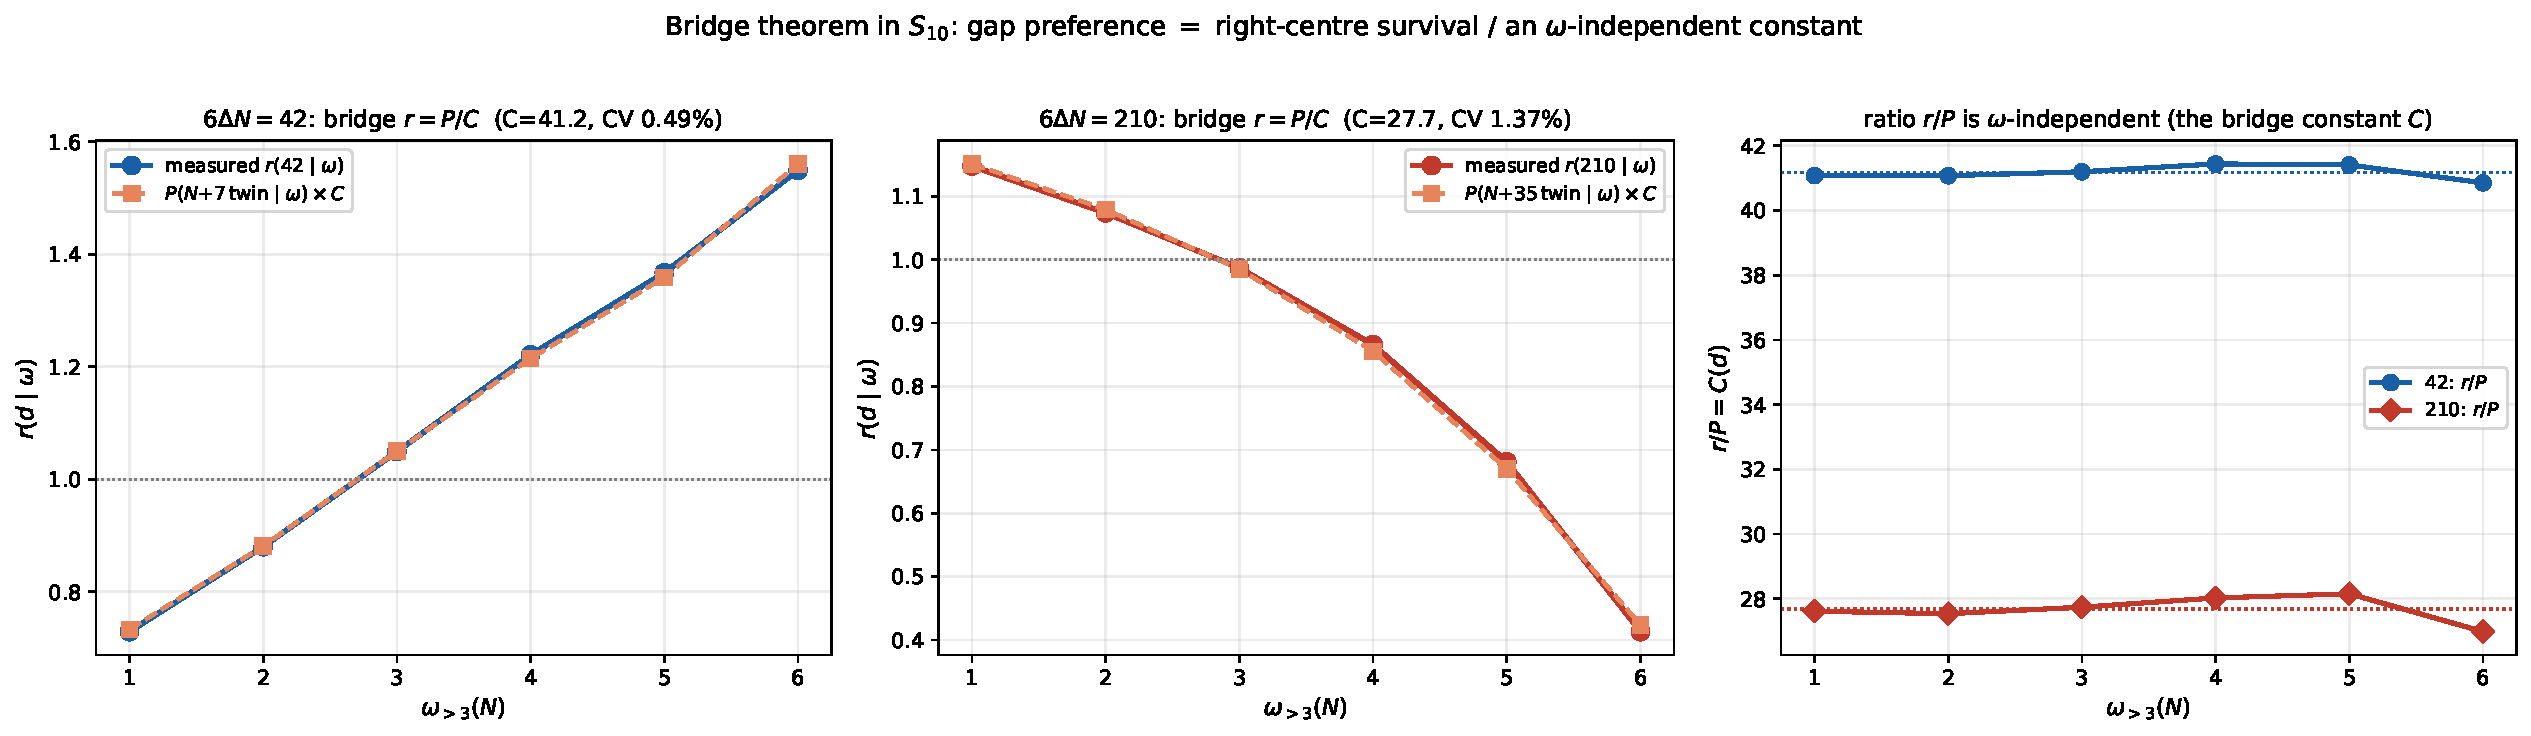
\includegraphics[width=\textwidth]{fig_paper6_bridge.pdf}
\caption{Bridge theorem in $S_{10}$. Left/centre: the measured gap preference $r$
(solid) and the right-centre survival rescaled by the constant, $P\times C$
(dashed), coincide for $42$ and $210$. Right: the ratio $r/P$ is flat in $\omega$
(the constant $C(d)$); the $210$ curve dips slightly at $\omega=6$.}
\label{fig:br}
\end{figure}

\section{Resolution of the $42$ residual}

Parts~II--IV reported the anomalous rise of $r(42\mid\omega)$ from $0.73$ to
$1.55$, which the single-centre second-order series of Part~IV could only half
explain. The bridge resolves it without any new mechanism. By
Theorem~\ref{thm:bridge},
\[
  r(42\mid\omega)=\frac{P(N{+}7\text{ twin}\mid\omega)}{41.17},
\]
so the rise of $r(42\mid\omega)$ \emph{is} the rise of the right-centre survival
$P(N{+}7\text{ twin}\mid\omega)$ from $0.018$ ($\omega{=}1$) to $0.038$
($\omega{=}6$), rescaled by a constant. And that rise is the cumulative
two-centre shield of Part~V: a factor-rich centre carries more small primes, each
contributing a modular-shift protection of the right centre (for $42$, dominated
by $q=5$, since $N{+}7\equiv N{+}2\pmod5$ lands the right centre on a safe
residue when $5\mid N$). The high-$\omega$ rise of $42$ is thus the bridge (a
normalisation) acting on the right-centre survival (driven up by the Part~V
shield). The chain is mechanistically complete:
\[
  \text{two-centre shield (V)}\ \Rightarrow\
  P(N{+}d\text{ twin}\mid\omega)\ \xrightarrow{\ \div C(d)\ (\text{VI})\ }\
  r(d\mid\omega).
\]

\section{What remains open}

Theorem~\ref{thm:bridge} converts the gap preference into the right-centre
survival, and Part~V explains the \emph{relative} ($\omega$-dependent) behaviour
of that survival through the shield $S(d,q)$. What is not yet in closed form is
the combination of the single-prime shields into the \emph{absolute} survival
$P(N{+}d\text{ twin}\mid\omega)$: a naive independent product over the centre's
primes overstates it (the cross-prime hedge of Part~V is non-multiplicative at
the level of full survival). The remaining problem is therefore narrower than at
any earlier stage.

\begin{quote}
\textbf{Open problem.} Give a closed-form expression for
$P(N{+}d\text{ twin}\mid N\text{ twin},\omega)$ in terms of the single-prime
two-centre shields $S(d,q)$ of Part~V, valid across $\omega$. Combined with the
bridge constant $C(d)$ of Theorem~\ref{thm:bridge}, this would yield a fully
closed-form $r(d\mid\omega)$.
\end{quote}

Also open is the value and the small $\omega=6$ deviation of $C(210)$: whether
$C(d)$ has an arithmetic expression in $d$, and whether the $1.37\%$ spread on
$210$ is a finite-size effect or a genuine breakdown of exact $\omega$-independence
at the sparsest stratum.

\section{Conclusion}

The bridge from the two-centre shield (Part~V) to the stratified gap preference
(Parts~II--IV) is a pure normalisation: $r(d\mid\omega)=P(N{+}d\text{ twin}\mid
\omega)/C(d)$ with an $\omega$-independent constant, holding to CV $0.49\%$ for
$42$ and $1.37\%$ for $210$ on $2.4\times10^{7}$ twin centres. This resolves the
$42$ residual that ran through Parts~II--V: its rise to $1.55$ is the rise of the
right-centre survival, itself the cumulative two-centre shield, rescaled by a
constant---no separate mechanism is needed. The six-part chain, from the local
density enrichment of Part~I to the gap-preference distribution here, now closes
mechanistically end to end, with a single narrower open problem: the closed-form
combination of single-prime shields into the absolute survival. As throughout,
no claim is made about the infinitude of twin primes or any $k$-tuple conjecture;
this is a measured, factor-resolved account of the conditional gap structure of
the $6N$ twin skeleton.

\paragraph{Data and code availability.}
The bridge measurement is openly available~\cite{repo}; the $S_{10}$ twin count
$23{,}988{,}173$ matches Part~I.

\begin{thebibliography}{9}
\bibitem{ChenI} R.~Chen, \emph{Prime distribution on the $6N$ skeleton} (Part~I),
Zenodo, doi:10.5281/zenodo.20470367 (2026).
\bibitem{ChenII} R.~Chen, \emph{Prime gaps on the $6N$ skeleton} (Part~II),
Zenodo, doi:10.5281/zenodo.20477664 (2026).
\bibitem{ChenIII} R.~Chen, \emph{A first-order conditional singular series}
(Part~III), Zenodo, doi:10.5281/zenodo.20498668 (2026).
\bibitem{ChenIV} R.~Chen, \emph{A second-order conditional singular series}
(Part~IV), Zenodo, doi:10.5281/zenodo.20500465 (2026).
\bibitem{ChenV} R.~Chen, \emph{A two-centre shield law} (Part~V), Zenodo,
doi:10.5281/zenodo.20510700 (2026).
\bibitem{repo} R.~Chen, \emph{$6N$ twin-prime bridge theorem: data and code},
\url{https://github.com/Ruqing1963/6N-twin-prime-bridge-theorem} (2026).
\end{thebibliography}

\end{document}
